\setlength{\footskip}{8mm}

\chapter{Dataset and Data Preparation}
\label{ch:Dataset}

%\section{Datasets and Data Preprocessing}
For our methodology, we focused on using a \cite{dataset}Urdu-Text: A Dataset and Benchmark for Urdu Text Detection and Recognition in Natural Scenes as it closely aligns with the requirements of our text detection approach. The natural scene dataset consists of diverse images with complex backgrounds, varying text sizes, orientations, and fonts, which pose challenges for accurate text detection.

To ensure compatibility with our methodology and to have precise ground truth annotations, we annotated the natural scene dataset ourselves. By creating polygon annotations, we were able to accurately outline the text regions in the images. This allowed us to train and evaluate our text detection model using the annotated dataset, ensuring that it aligns with the specific requirements and objectives of our methodology.

By annotating the dataset ourselves, we had control over the annotation quality and consistency, ensuring that the annotations precisely captured the boundaries of the text regions. This annotated dataset serves as a valuable resource for training and evaluating our text detection model, enabling us to assess its performance and validate the effectiveness of our methodology in the context of natural scene images.

\section{Dataset Description}
The Urdu-Text dataset consists of 1400 scene images that contain a mixture of Urdu, English, Sindhi, and Arabic text instances. These text instances encompass various forms, including machine-printed text on shop names, advertisement banners, street names, as well as handwritten text on walls and hoardings. The dataset is divided into 1000 samples for training and 400 samples for testing. Within the dataset, there are a total of 13788 labeled text regions, each represented by a quadrilateral bounding box that indicates the location of the text instance. The annotations also include information about the script type and the transcription of the text. Here is a glimpse of a dataset in Figure ~\ref{fig:data}

\begin{figure}[htp]
  \centering
  \begin{minipage}{0.4\textwidth}
    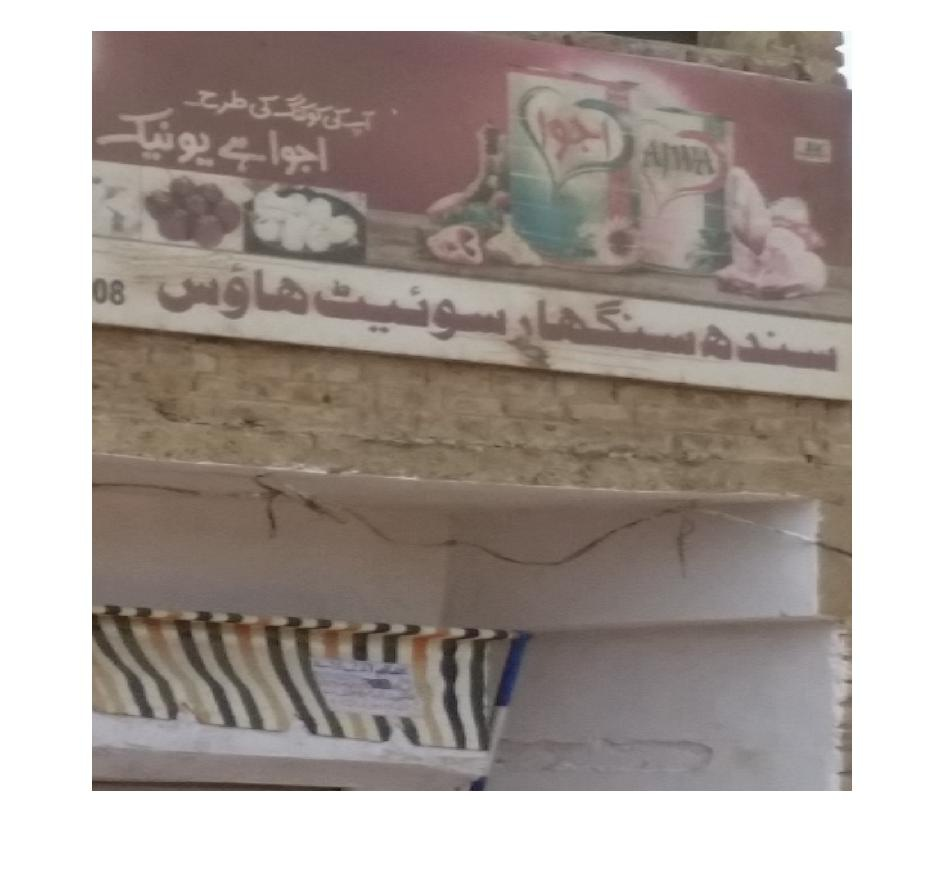
\includegraphics[width=\linewidth]{ITU-Thesis-LaTeX-Template-Updated/figures/data1.png}
    \text{Image}
  \end{minipage}
  \begin{minipage}{0.4\textwidth}
    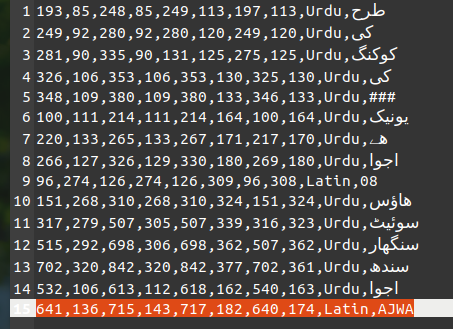
\includegraphics[width=\linewidth]{ITU-Thesis-LaTeX-Template-Updated/figures/Picture2.png}
    \text{Quadrilateral Annotation}
  \end{minipage}
  \caption{Benchmark Dataset Description}
  \label{fig:data}
\end{figure}
\FloatBarrier

\section{Model Specific Data preprocessing}
Data preprocessing constitutes a foundational stage in our text detection pipeline, playing a pivotal role in shaping the input data to align with the specific requirements of our chosen models: Faster R-CNN, YOLO (You Only Look Once), and models leveraging Graph Convolutional Networks (GCN). This section elucidates the model-specific data preprocessing strategies deployed to optimize data compatibility and feature extraction.

\subsection{YOLO Data Preprocessing}
The YOLO model relies on bounding boxes to annotate objects in images. However, our original dataset employs quadrilateral annotations for text instances. To adapt our dataset for YOLO-based text detection, we executed the following data preprocessing steps:

\textbf{1. Quadrilateral to Bounding Box Conversion:} For each quadrilateral annotation, we calculated the coordinates of the minimum and maximum x and y values among the four corners of the quadrilateral. These minimum and maximum values were then utilized to determine the coordinates of the bounding box that fully encompasses the quadrilateral.

\textbf{2. Coordinate Normalization:} YOLO employs normalized coordinates, which are relative to the dimensions of the image. We normalized the coordinates of the bounding boxes by dividing them by the width and height of the respective image. The normalization process ensured that the coordinates were scaled appropriately for YOLO's input requirements. Specifically, the following equations were applied:

   \begin{equation}
    \text{normalized\_x\_center} = \frac{x_{\text{min}} + x_{\text{max}}}{2 \times \text{width}}
    \end{equation}
    
    \begin{equation}
    \text{normalized\_y\_center} = \frac{y_{\text{min}} + y_{\text{max}}}{2 \times \text{height}}
    \end{equation}
    
    \begin{equation}
    \text{normalized\_width} = \frac{x_{\text{max}} - x_{\text{min}}}{\text{width}}
    \end{equation}
    
    \begin{equation}
    \text{normalized\_height} = \frac{y_{\text{max}} - y_{\text{min}}}{\text{height}}
   \end{equation}


\textbf{3. Labeling and Formatting:} For each object in the image, we created a YOLO annotation line in the following format: \\

\text{class\_id} \quad \text{normalized\_x\_center} \quad \text{normalized\_y\_center} \quad \text{normalized\_width} \quad \text{normalized\_height}

   \begin{align*}
    \text{class\_id} & : \text{Represents the class label of the object.} \\
    \text{normalized\_x\_center} & : \text{Normalized x-coordinate of the center of the bounding box.} \\
    \text{normalized\_y\_center} & : \text{Normalized y-coordinate of the center of the bounding box.} \\
    \text{normalized\_width} & : \text{Normalized width of the bounding box.} \\
    \text{normalized\_height} & : \text{Normalized height of the bounding box.} 
    \end{align*}

   Each object in the image was represented by a separate line in the YOLO annotation file.

\textbf{4. Annotation File Creation:} Following the aforementioned steps, we created YOLO annotation files for each image in the dataset. These annotation files were saved with the same name as the corresponding image but with a .txt extension. Each line in the annotation file represented an object in the image, following the YOLO annotation format.

The data preprocessing steps outlined above successfully transformed our dataset with quadrilateral annotations into a format suitable for YOLO-based text detection as in the Figure ~\ref{fig:data_yolo}. These adapted annotations were subsequently used to train our YOLO text detection model.

\begin{figure}[htp]
  \centering
  \begin{minipage}{0.4\textwidth}
    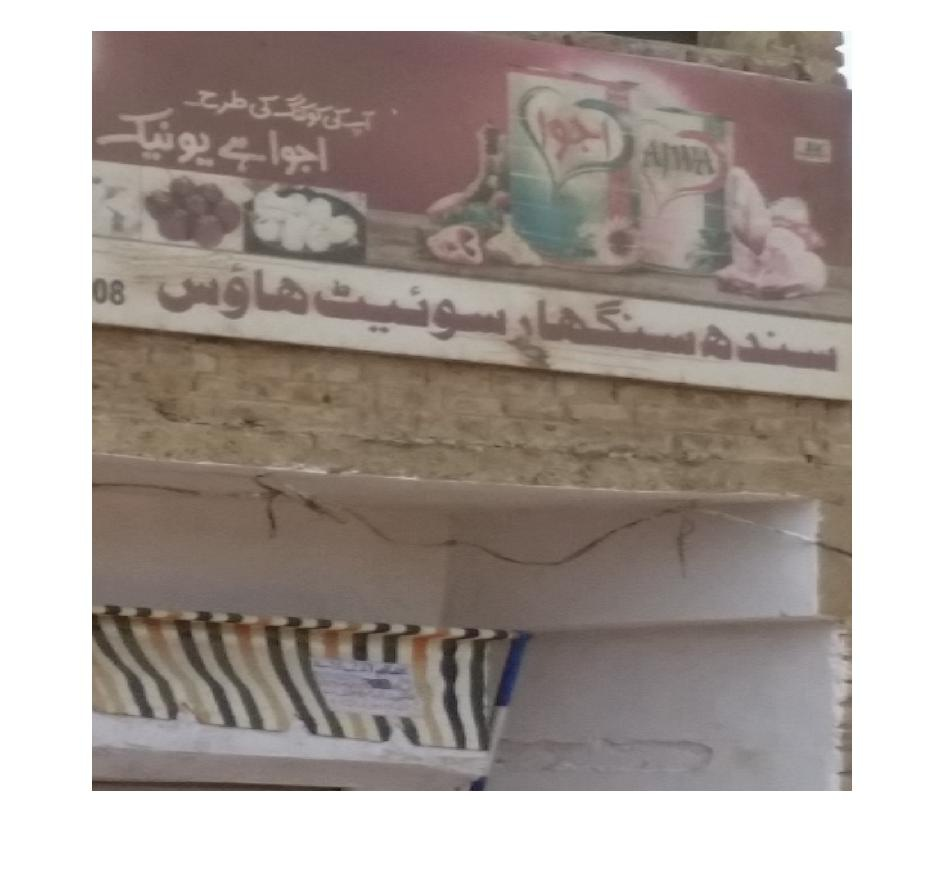
\includegraphics[width=\linewidth]{ITU-Thesis-LaTeX-Template-Updated/figures/data1.png}
    \text{Image}
  \end{minipage}
  \begin{minipage}{0.4\textwidth}
    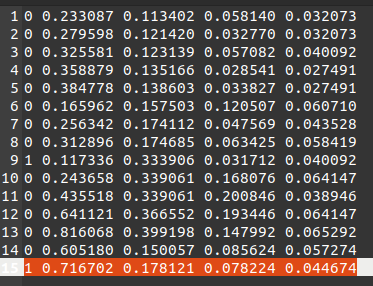
\includegraphics[width=\linewidth]{ITU-Thesis-LaTeX-Template-Updated/figures/Picture3.png}
    \text{YOLO Bounding Box Annotation}
  \end{minipage}
  \caption{YOLO Compatible Annotations}
  \label{fig:data_yolo}
\end{figure}
\FloatBarrier

\subsection{Data Preprocessing for Faster R-CNN}

Data preprocessing is a crucial preparatory step in the utilization of the Faster R-CNN architecture for text detection. In this section, we elaborate on the essential procedures undertaken to transform our dataset into a format compatible with Faster R-CNN. This preparation includes the conversion of bounding box annotations from YOLO format to the COCO format, which is commonly employed for Faster R-CNN-based object detection tasks.

\textbf{1. Class Mapping:} The first step in adapting our dataset for Faster R-CNN involves ensuring consistency in class labels between the original YOLO dataset and the COCO dataset. We establish a one-to-one mapping between the class labels, allowing for seamless transition and interpretation of annotations within the Faster R-CNN framework.

\textbf{2. Bounding Box Conversion: } The representation of bounding boxes plays a pivotal role in compatibility between YOLO and Faster R-CNN. While YOLO relies on normalized coordinates for bounding boxes, Faster R-CNN employs the COCO format, necessitating the transformation of coordinates. The conversion from YOLO to COCO format is accomplished through the following formulas:

\begin{equation}
x_{\text{min}} = (\text{normalized\_x\_center} - 0.5 \times \text{normalized\_width}) \times \text{image\_width}
\end{equation}

\begin{equation}
y_{\text{min}} = (\text{normalized\_y\_center} - 0.5 \times \text{normalized\_height}) \times \text{image\_height}
\end{equation}

\begin{equation}
\text{width} = \text{normalized\_width} \times \text{image\_width}
\end{equation}

\begin{equation}
\text{height} = \text{normalized\_height} \times \text{image\_height}
\end{equation}

Here, $\text{normalized\_x\_center}$ and $\text{normalized\_y\_center}$ denote the normalized coordinates of the center of a YOLO bounding box, while $\text{normalized\_width}$ and $\text{normalized\_height}$ represent the normalized width and height of the bounding box. $\text{image\_width}$ and $\text{image\_height}$ refer to the dimensions of the original image.

\textbf{3. Image Metadata} In the COCO format, each annotation is enriched with crucial metadata. This metadata encompasses unique image identifiers (IDs), file names, and image dimensions. The inclusion of this information ensures comprehensive compatibility with Faster R-CNN's data loading pipeline. You can see this in a Figure~\ref{fig:data_fasterRCNN}

\begin{figure}[htp]
  \centering
  \begin{minipage}{0.4\textwidth}
    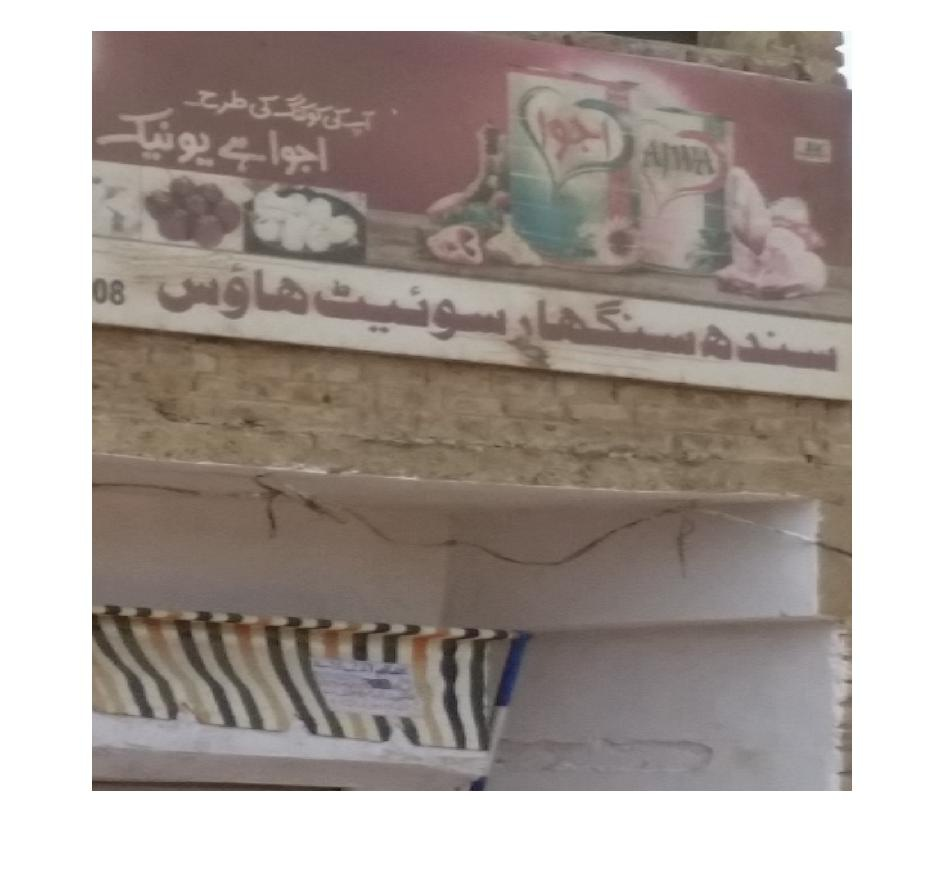
\includegraphics[width=\linewidth]{ITU-Thesis-LaTeX-Template-Updated/figures/data1.png}
    \text{Image}
  \end{minipage}
  \begin{minipage}{0.4\textwidth}
    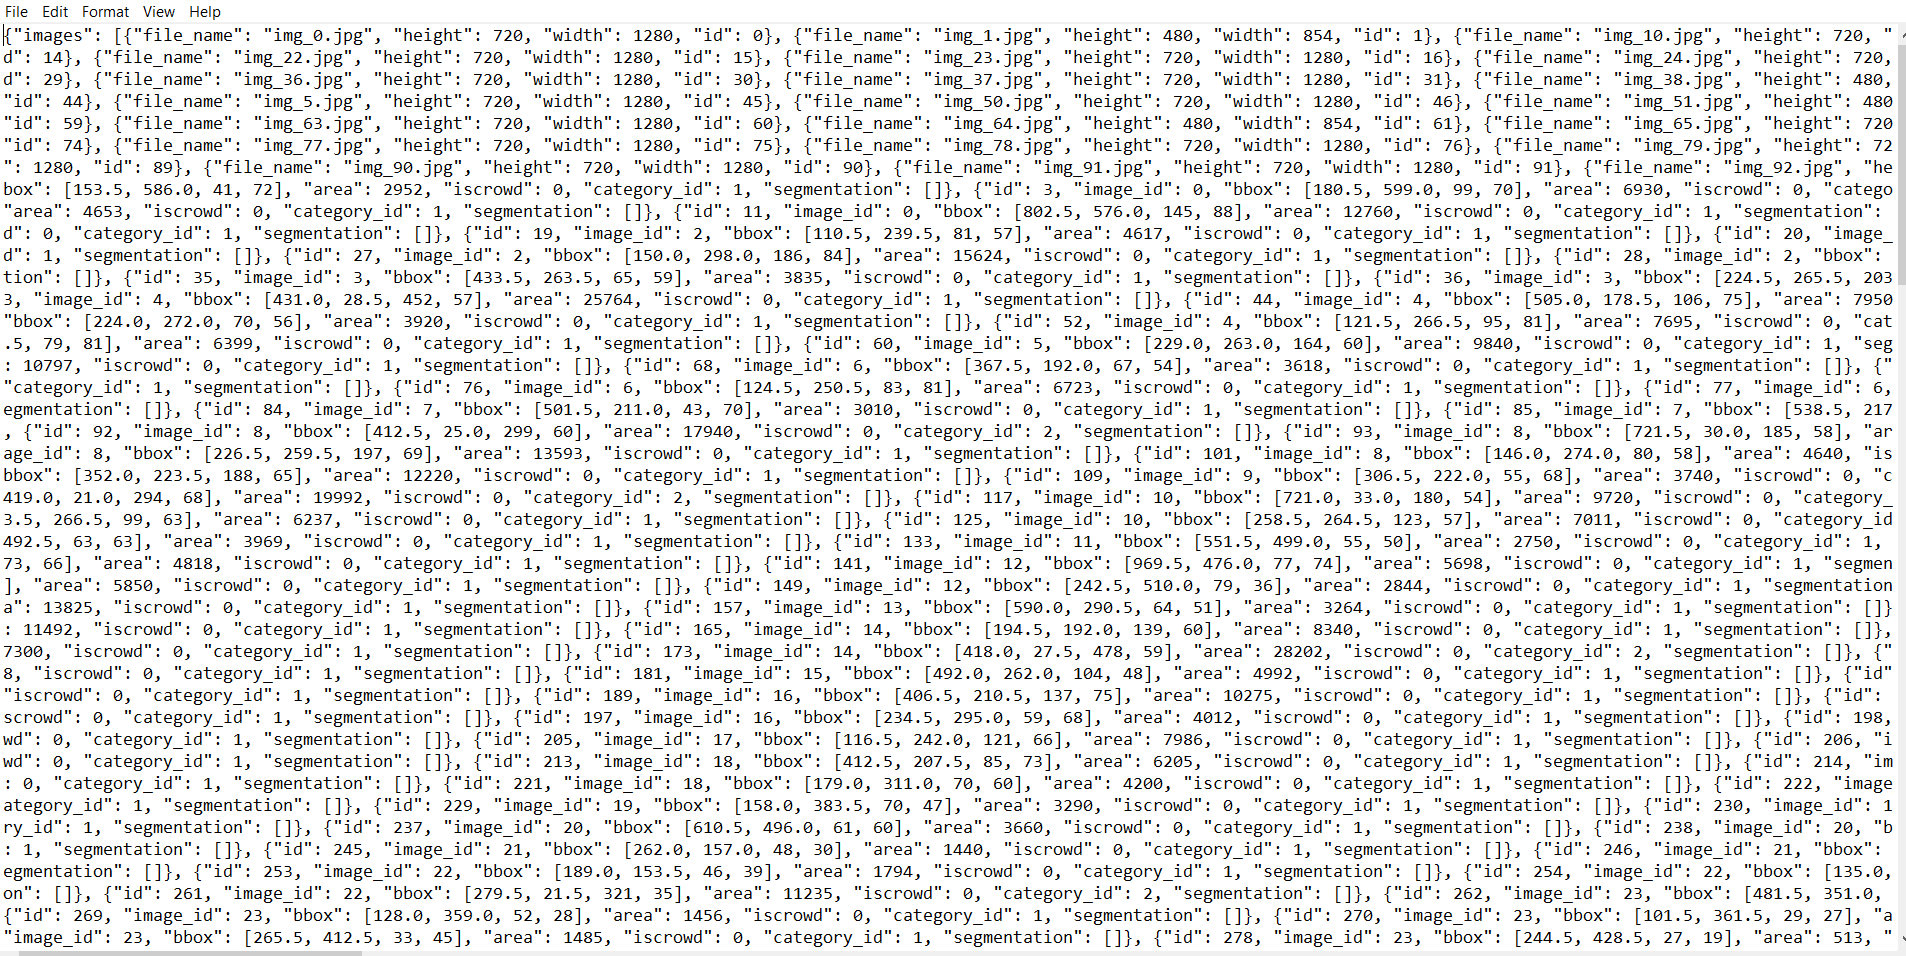
\includegraphics[width=\linewidth]{ITU-Thesis-LaTeX-Template-Updated/figures/Picture4.png}
    \text{Cocoo Annotation}
  \end{minipage}
  \caption{FasterRCNN Compatible Annotations}
  \label{fig:data_fasterRCNN}
\end{figure}
\FloatBarrier

With these meticulous preprocessing steps, our dataset is now prepared in the COCO format, rendering it compatible with the Faster R-CNN architecture. The resulting dataset retains essential attributes, including class labels and precise bounding box coordinates, enabling the application of Faster R-CNN for text detection tasks.

This conversion process not only facilitates the utilization of Faster R-CNN but also allows for comparative analyses between YOLO and Faster R-CNN, further enhancing the depth and comprehensiveness of our research. This difference can be elaborated visually too like this in Figure~\ref{fig:yolovscocoo}

\begin{figure}[htp] 
  \centering
  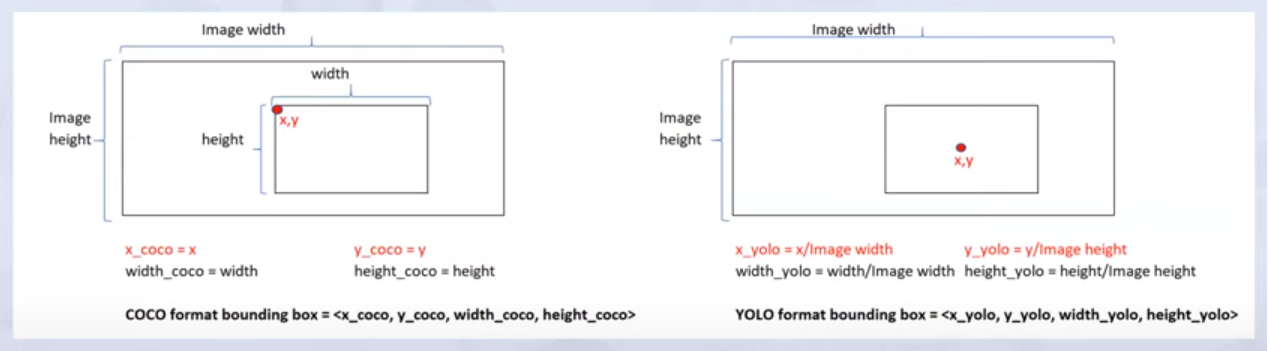
\includegraphics[width=6in]{ITU-Thesis-LaTeX-Template-Updated/figures/yolovsc.png}
  \caption{YOLO Vs Cocoo}
  \label{fig:yolovscocoo}
\end{figure}
\FloatBarrier

\subsection{Data Preprocessing for Our Framework}
The preparation of input data forms a cornerstone in the development of any robust text detection framework. In our journey to create a highly effective text detection system, we initially encountered a diverse array of annotation types, including quadrilateral, YOLO, and COCO formats. However, our framework's pivotal component, the Graph Convolutional Network (GCN), presented a distinctive requirement. GCN, designed to discern intricate spatial relationships and patterns within images, demanded a specialized form of data representation - polygon annotations. These polygon annotations, unlike their counterparts, encapsulate the precise geometric attributes of text instances. To fulfill this need, we undertook the task of annotating our data by ourselves, meticulously creating polygon annotations to enrich the dataset. Furthermore, recognizing the significance of data diversity and scale, we ventured into generating a synthetic dataset, a process we will elaborate on in subsequent sections. These combined efforts, annotating and synthesizing, serve as the bedrock of our text detection framework, enhancing its adaptability and robustness for a multitude of real-world scenarios. In the following sections, we will delve into the intricacies of how we accomplished these tasks, shedding light on the methodology behind the creation of our polygon annotations for our synthetic dataset.

\subsubsection{Our Synthetic Dataset}
In our study, we utilized images from the Urdu-Text dataset, which originally provided quadrilateral annotations for the text regions in the natural scene images. However, we found that using polygon annotations instead of quadrilaterals offered several advantages in the context of our research.

Firstly, polygon annotations provide a more accurate representation of the actual shape of the text region. By annotating the text regions with polygons, we were able to better capture irregular shapes and contours that might not be adequately represented by quadrilaterals. This improved accuracy is crucial for tasks such as text detection and recognition, where precise localization of the text is essential.

Secondly, polygon annotations offer greater flexibility in capturing complex text regions. Text instances in natural scene images can exhibit diverse shapes, including curved or skewed boundaries. Polygon annotations allow us to delineate these intricate shapes more effectively, enabling better modeling and analysis of the text regions.

Furthermore, polygon annotations facilitate a more natural and intuitive representation of text regions. As polygons closely follow the contours of the text, they provide a clearer visual depiction of the text boundaries. This visual clarity can aid researchers and practitioners in understanding the structure and layout of text instances within the scene images.

Overall, the use of polygon annotations in our study improved the accuracy, flexibility, and visual representation of the text regions in the Urdu-Text dataset. This enhancement allows for more reliable and precise analysis of the text, ultimately contributing to the effectiveness of our research in text detection and related tasks.

\section{Polygons Generations}
In order to obtain polygon annotations for the text regions in the Urdu-Text dataset, we made use of the V7labs annotation tool. Using this tool, we manually labeled the text instances in the dataset by tracing the contours of the text regions. The output of this annotation process was a set of segmentation masks, which represented the pixel-wise delineation of the text regions.

After obtaining the segmentation masks using V7labs, we performed preprocessing steps using the OpenCV library. Specifically, we utilized the findContours function from OpenCV, which enabled us to extract the contours from the segmentation masks.

The findContours function in OpenCV analyzes the binary image (segmentation mask) and identifies the contours of connected components, in this case, the text regions. It traces the boundaries of these connected components, providing a set of contours that represent the shape of the text regions.

By extracting the contours using the findContours function, we obtained a collection of boundary points that formed the outlines of the text regions. These boundary points allowed us to create polygons that accurately defined the boundaries of the text instances.

The usage of the findContours function in OpenCV for preprocessing the segmentation masks and extracting the contours was instrumental in obtaining polygon annotations for the text regions in the Urdu-Text dataset. The result of this effort is shown below in Figure ~\ref{fig:data_polygons}. These polygon annotations offer a more precise and detailed representation of the text regions, enabling advanced analysis and research in text detection and recognition.

\begin{figure}[htp]
  \centering
  \begin{minipage}{0.4\textwidth}
    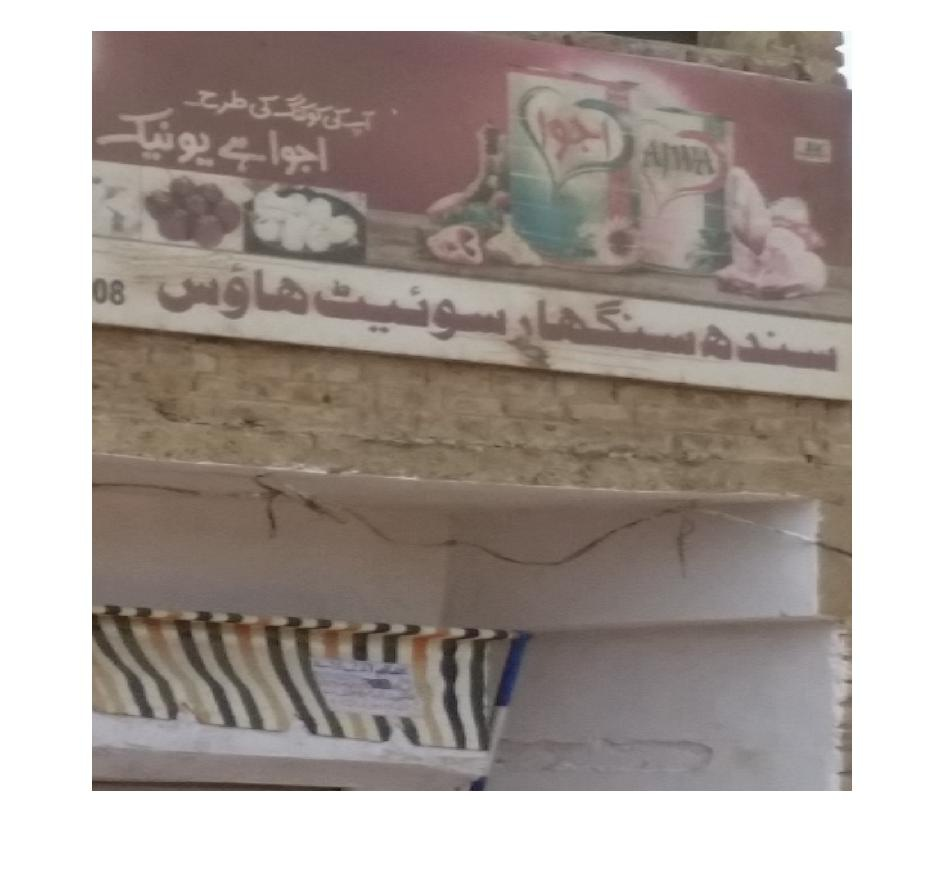
\includegraphics[width=\linewidth]{ITU-Thesis-LaTeX-Template-Updated/figures/data1.png}
    \text{Image}
  \end{minipage}
  \begin{minipage}{0.5\textwidth}
    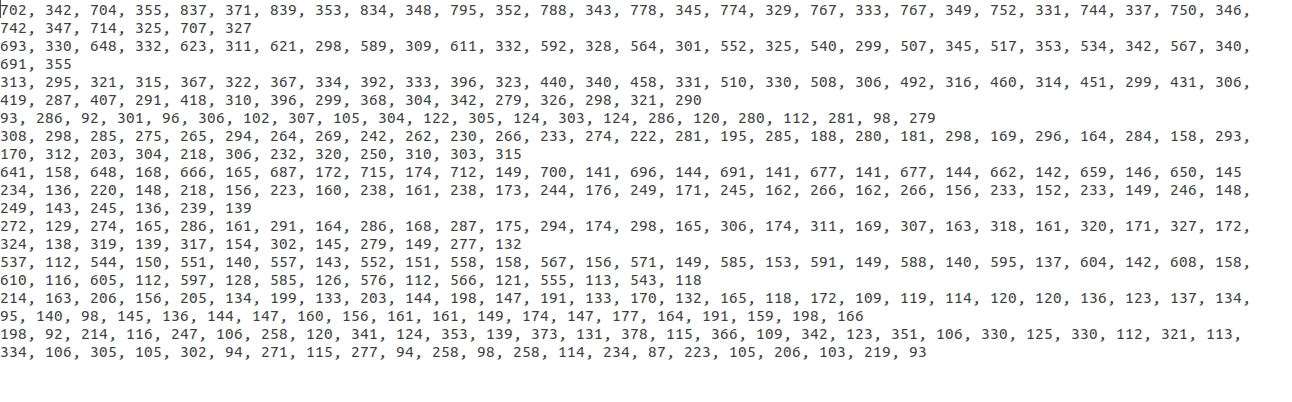
\includegraphics[width=\linewidth]{ITU-Thesis-LaTeX-Template-Updated/figures/polygons.png}
    \text{Polygon Annotation}
  \end{minipage}
  \caption{Polygons Annotations}
  \label{fig:data_polygons}
\end{figure}
\FloatBarrier

\FloatBarrier